	\documentclass[10pt,oneside]{CBFT_book}
	% Algunos paquetes
	\usepackage{amssymb}
	\usepackage{amsmath}
	\usepackage{graphicx}
	\usepackage{libertine}
	\usepackage[bold-style=TeX]{unicode-math}
	\usepackage{lipsum}

	\usepackage{natbib}
	\setcitestyle{square}

	\usepackage{polyglossia}
	\setdefaultlanguage{spanish}


	\usepackage{CBFT.estilo} % Cargo la hoja de estilo

	% Tipografías
	% \setromanfont[Mapping=tex-text]{Linux Libertine O}
	% \setsansfont[Mapping=tex-text]{DejaVu Sans}
	% \setmonofont[Mapping=tex-text]{DejaVu Sans Mono}

	%===================================================================
	%	DOCUMENTO PROPIAMENTE DICHO
	%===================================================================

\begin{document}

\chapter{Sistemas rotantes}

% =================================================================================================
\section{Sistemas rotantes}
% =================================================================================================

Consideramos un sistema inercial $X,Y,Z$ y un sistema rotante $X',Y',Z'$

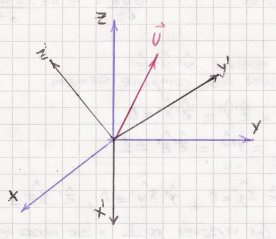
\includegraphics[scale=0.5]{images/fig_mc_rotantes1.jpg}

El cambio de coordenadas entre los dos sistemas adopta la forma 
\[
	\vb{U}' = A \vb{U}
\]
donde $A$ es la matriz del cambio de coordenadas. Transformación ortogonal.

Para una rotación plana, en 2D, se tiene explícitamente
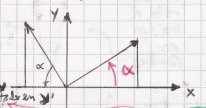
\includegraphics[scale=0.5]{images/fig_mc_rotantes2.jpg}
\[
	\begin{pmatrix}
	x' \\
	y'
	\end{pmatrix} =
	\begin{pmatrix}
	 \cos \alpha & \sin \alpha \\
	 -\sin \alpha & \cos \alpha 
	\end{pmatrix} 
	\begin{pmatrix}
	 x \\
	 y
	\end{pmatrix} 
\]
donde cada elemento de la matriz de transformación es la proyección de un versor en los ejes
primados.
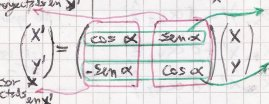
\includegraphics[scale=0.5]{images/fig_mc_rotantes3.jpg}

Las condiciones de ortogonalidad implican que 
\begin{itemize}
 \item Las columnas tienen norma 1.
 \item Las filas tienen norma 1.
 \item El producto escalar de dos filas o dos columnas es nulo.
\end{itemize}

Si 
\[
	A = \begin{pmatrix}
		a_{11} & a_{12} & a_{13} \\
		a_{21} & a_{22} & a_{23} \\
		a_{31} & a_{31} & a_{33} 
	    \end{pmatrix},
\]
donde cada uno de estos $ a_{ij} $ puede depender del tiempo. Entonces,
\[
	\sum_{j=1}^3 a_{ij} a_{lj} = \delta_{il} \qquad \qquad 
	\sum_{j=1}^3 a_{ji} a_{jl} = \delta_{il} 
\]

Una rotación infinitesimal puede describirse con un vector que sí son conmutativas.
Para un observador rotando en $X'Y'Z'$ los versores $x,y,z$ se mueven con el tiempo.

\subsection{Recordemos la transformación de Galileo}
\[
	\vb{x} = \vb{X} + \vb{r}' \qquad \qquad 
	\vb{v} = \vb{V} + \vb{v}'
\]
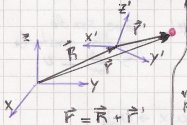
\includegraphics[scale=0.5]{images/fig_mc_rotantes_galileo.jpg}

Entonces la derivada temporal de uno u otro vector tienen diferente aspecto puesto 
que hay versores que varían con el tiempo, y otros que no. En efecto
\[
	\dtot{\vb{U}}{t} = \dtot{}{t} \left( U_x \hat{x} + U_y \hat{y} + U_z \hat{z} \right) =
	\dtot{U_x}{t}\hat{x} + \dtot{U_y}{t} \hat{y} + \dtot{U_z}{t} \hat{z},
\]
tiene versores independientes del tiempo mientras que 
\[
	\dtot{\vb{U}'}{t} = \dtot{}{t} \left( U_x' \hat{x}' + U_y' \hat{y}' + U_z' \hat{z}' \right) =
	\dtot{U_x'}{t}\hat{x}' + \dtot{U_y'}{t} \hat{y}' + \dtot{U_z'}{t} \hat{z}' +
	U_x'\dtot{\hat{x}'}{t} + U_y'\dtot{\hat{y}'}{t} + U_z' \dtot{\hat{z}'}{t} 
\]
no los tiene y deben ser derivados.

No obstante, al variar los versores $\hat{x}',\hat{y}',\hat{z}'$, dada su ortogonalidad,
deben cumplirse siempre
\be
	\hat{x}' \hat{y}' = \hat{z}' \hat{y}' = \hat{z}' \hat{x}' = 0
	\label{escalar_versores_1}
\ee
\be
	\hat{x}' \hat{x}' = \hat{y}' \hat{y}' = \hat{z}' \hat{z}' = 1
	\label{escalar_versores_2}
\ee

De la segunda ecuación anterior \eqref{escalar_versores_2} surge que 
\[
	\hat{x}' \delta {x}' = 0, \; \hat{y}' \delta {y}' = be0, \;  \hat{z}' \delta {z}' = 0,
\]
la variación de los versores es perpendicular a los versores mismos porque al rotar no se varía
el módulo; como son de módulo constante,
\[
	\dtot{U}{t} \perp U
\]

Ilustración: si solo rota, no varía el módulo

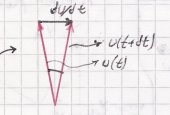
\includegraphics[scale=0.5]{images/fig_mc_rotantes4.jpg}

Las variaciones pueden escribirse así
\[
	\begin{cases}
	\delta \hat{x}' = \delta \alpha_{xy} \hat{y}' + \delta \alpha_{xz} \hat{z}' \\
	\delta \hat{y}' = \delta \alpha_{yx} \hat{x}' + \delta \alpha_{yz} \hat{z}' \\
	\delta \hat{z}' = \delta \alpha_{zx} \hat{x}' + \delta \alpha_{zy} \hat{y}'
	\end{cases}
\]
donde vemos que no aparec $x$ en la $\delta x$ puesto que es perpendicular [?]

Utilizando la ecuación \eqref{escalar_versores_1}
\[
	\delta( \hat{x}' \hat{z}') = \delta \hat{x}' \hat{z}' + \hat{x}' \delta \hat{z}' = 0
\]
donde podemos identificar $\delta\alpha_{xz}=\delta \hat{x}'$ y $\delta\alpha_{zx}=\delta \hat{z}'$.
Los vínculos surgidos de dicha ecuación son 
\[
	\delta\alpha_{xz} = -\delta\alpha_{xz} \qquad 
	\delta\alpha_{yx} = -\delta\alpha_{xy} \qquad 
	\delta\alpha_{yz} = -\delta\alpha_{zy} 
\]
Ahora solo necesitaremos tres números para la rotación 3D
Si definimos:
\[
	\delta\alpha_{xz} \equiv -\delta\alpha_{y} \qquad 
	\delta\alpha_{xy} \equiv \delta\alpha_{z} \qquad 
	\delta\alpha_{zy} \equiv -\delta\alpha_{x} 
\]
se tiene 
\[
	\begin{cases}
	\delta \hat{x}' = \delta \alpha_{z} \hat{y}' - \delta \alpha_{y} \hat{z}' \\
	\delta \hat{y}' = -\delta \alpha_{z} \hat{x}' + \delta \alpha_{x} \hat{z}' \\
	\delta \hat{z}' = \delta \alpha_{y} \hat{x}' - \delta \alpha_{x} \hat{y}'
	\end{cases}
\]

Supongamos rotar en torno a $\hat{z}$

% \bibliographystyle{CBFT-apa-good}	% (uses file "apa-good.bst")
% \bibliography{CBFT.Referencias} % La base de datos bibliográfica

\end{document}
